%%%%%%%%%%%%%%%%%%%%%%%%%%%%%%%%%%%%%%%%%%%%%%%%%%%%%%%
%%%%% Sec: Light sources modeling  %%%%%
%%%%%%%%%%%%%%%%%%%%%%%%%%%%%%%%%%%%%%%%%%%%%%%%%%%%%%%
\section{Light sources modeling}
\label{sec:light_models}

The prevalent approach to modeling light sources such as galaxies involves using a parametric profile $(R)$, where $R$ represents a measure of distance from the center of the object. These models often presuppose an excessively idealized level of symmetry, yet offer the advantage of being straightforward to define and apply. When building galaxy components, it is generally assumed that the profiles exhibit elliptical symmetry \citep{peng_detailed_2002,peng_detailed_2010}, and therefore $R$ represents the elliptical radius
\be
\label{eq:4.13}
R (\vec{x}^\prime) = \sqrt{{x_1^\prime}^2 + {x_2^\prime / q}^2}
\ee
of a source with an axis ratio $q$. The coordinate system $({x_1^\prime} , {x_2^\prime})$ of the source can be rotated by the \emph{position angle} $\varphi$ with respect to the coordinate system $(x_1 , x_2)$ of the observation. The resulting isophotes\footnote{Curves of constant surface brightness.} of the surface brightness distribution of such an elliptical source are ellipses with semi-major axis $R/q$, semi-minor axis $R$ and orientation $\varphi$ with respect to the $x_1$ axis of observation.


%%%%%%%%%%%%%%%%%%%%%%%%%%%%%%%%%%%%%%%%%%%%%%%%%%%%%%%
%%%%% SubSec: Sérsic profile %%%%%
%%%%%%%%%%%%%%%%%%%%%%%%%%%%%%%%%%%%%%%%%%%%%%%%%%%%%%%
\subsection{Sérsic profile}
\label{subsec:sersic}
The most common model to describe elliptical surface brightness distributions is the \emph{Sérsic law} \citep{sersic_influence_1963,sersic_atlas_1968}, which is given by the exponential
\be
\label{eq:4.14}
I(R) = I_e \exp \bc{- b_n \bs{\bp{\frac{R}{R_{e}}}^{\frac{1}{n}} - 1}} \,,
\ee
where $I_e$ is the surface brightness at the effective radius\footnote{Also called the half-light radius, the radius within which half of the galaxy’s luminosity is contained.} $R_e$ and $n>0$ is called the \emph{Sérsic index}, which characterizes the slope of the profile. The function $b_n$ depends only on the Sérsic index and is defined by
\be
\label{eq:4.15}
\g (2n, b_n) = \frac{1}{2} \G(2n) \,,
\ee
where $\G$, $\g$ are, respectively, the Gamma function and the incomplete Gamma function. It can be shown \citep{ciotti_stellar_1991,ciotti_analytical_1999} that, for a Sérsic index in the range $0.5 \leq n \lesssim 8$, $b_n$ can be approximated by
\be
\label{eq:4.16}
b_n \approx 2n - \frac{1}{3} + \frac{4}{405n} \approx 1.9992n - 0.3271 \,.
\ee
With this, the profile is now fully determined by the seven parameters for position $x_1$, $x_2$, effective radius $R_e$, Sérsic index $n$, intensity at the effective radius $I_e$, axis ratio $q$ and position angle $\varphi$.

The Sérsic profile is a versatile model; by varying $n$ it is possible to obtain many of the classical galaxy profiles as special cases, such as Gaussian profiles ($n = 0.5$), exponential profiles ($n = 1$) and de Vaucouleurs \citep{de_vaucouleurs_recherches_1948} profiles ($n = 4$). 

\begin{figure}
    \centering
    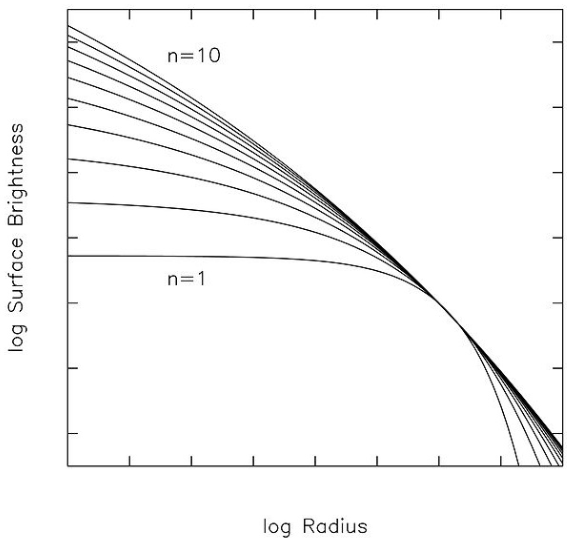
\includegraphics[width=0.65\linewidth, keepaspectratio]{img//chapter4/sersic_n.png}
    \caption[Sérsic profiles for different values of $n$]{Sérsic profiles for different values of $n$. On average, $n \approx 2-10$ for bulges and elliptical galaxies, $n\approx 1$ for disk galaxies and $n \leq 0.5$ for bars and stellar clumps.\\\small{Credits: \cite{burke_assembly_2013}.}}
    \label{fig:sersic_n}
\end{figure}


%%%%%%%%%%%%%%%%%%%%%%%%%%%%%%%%%%%%%%%%%%%%%%%%%%%%%%%
%%%%% SubSec: Core-Sérsic profile %%%%%
%%%%%%%%%%%%%%%%%%%%%%%%%%%%%%%%%%%%%%%%%%%%%%%%%%%%%%%
\subsection{Core-Sérsic profile}
\label{subsec:core_sersic}
An extension of the Sérsic profile has been developed by \cite{graham_new_2003,graham_inner_2004,trujillo_evidence_2004} to better reproduce the observed radial profiles of surface brightness. This model consists of a power law to model the inner radii and a Sérsic function to describe the outer stellar distribution. It is given by
\be
\label{eq:4.17}
I(R) = I^\prime \bs{1 + \bp{\frac{R_b}{R}}^\a}^{\g / \a} \exp{-b_n \bs{\frac{R^\a + R_b^\a}{R_e^\a}}^{1 / (\a n)}} \,,
\ee
where $R_b$ is the break-radius separating the inner power law with logarithmic slope $\g$ from the outer Sérsic profile with slope $n$. The intensity $I_b$ at the break-radius $R_b$ can be evaluated from the expression
\be
\label{eq:4.18}
I^\prime = I_b 2^{- \g / \a} \exp{b_n \bs{\frac{2^{1 / \a} R_b}{R_e}}^{1 / n}} \,.
\ee
The parameter $\a$ controls the sharpness of the transition between the inner (power law) and outer (Sérsic) regimes, with higher values indicating sharper transitions (\cref{fig:core_sersic}).

In this case, the number of parameters becomes larger to include the inner-outer change of regime: the profile is fully determined by ten parameters: for position $x_1$, $x_2$, effective radius $R_e$, Sérsic index $n$, intensity $I_b$ at the break-radius $R_b$, slope of the inner power law $\g$, sharpness of the transition $\a$, axis ratio $q$ and position angle $\varphi$.

\begin{figure}
    \centering
    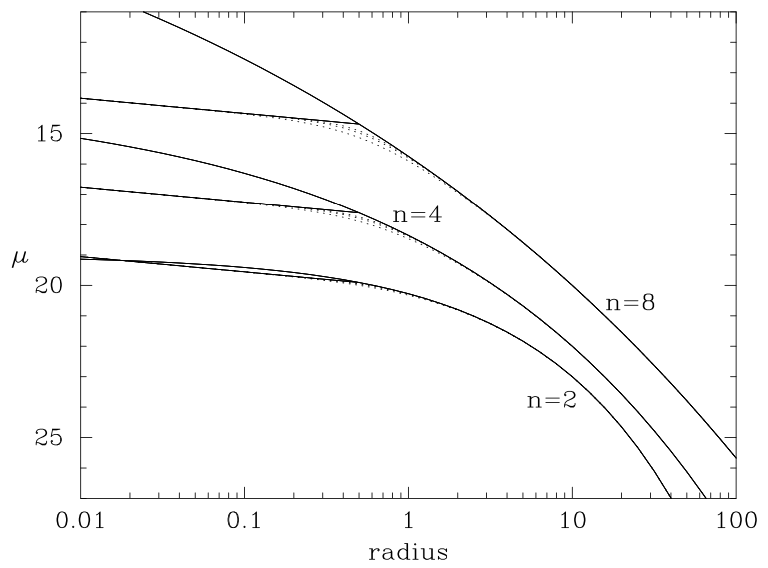
\includegraphics[width=0.7\linewidth, keepaspectratio]{img//chapter4/core_sersic.png}
    \caption[Core-Sérsic profiles for different values of $\a$]{Different core-Sérsic profiles illustrated by the dotted curves for a range of structural parameters. Profiles with values of $\a$ equal to 2, 3, and 4 are shown, the latter giving the sharpest transition. In all models $R_e = \SI{10}{\arcsec}$, $R_b = \SI{0.5}{\arcsec}$, and $\g = 0.2$. For comparison, an inner power law with slope equal to $-0.2$ is shown (diagonal solid lines), as are Sérsic profiles (solid curves) having the same Sérsic shape index $n$.\\\small{Credits: \cite{graham_new_2003}.}}
    \label{fig:core_sersic}
\end{figure}


%%%%%%%%%%%%%%%%%%%%%%%%%%%%%%%%%%%%%%%%%%%%%%%%%%%%%%%
%%%%% SubSec: Sky component  %%%%%
%%%%%%%%%%%%%%%%%%%%%%%%%%%%%%%%%%%%%%%%%%%%%%%%%%%%%%%
\subsection{Sky component}
\label{subsec:sky}
Observations usually include a diffuse distribution of light known as the \emph{sky background}, which must be considered in the reconstruction process. The most basic model for this sky component is a flat surface brightness distribution, characterized by a constant value or a fixed gradient along the $x_1$ and $x_2$ axes of the lens plane. Even if the diffuse background has been removed during a pre-processing step, incorporating a sky component as a free element in the model is advisable. Distinguishing between sky and actual signal is challenging, and any over- or underestimation of the subtracted light can have a considerable impact on the reconstruction outcomes.

%%%%%%%%%%%%%%%%%%%%%%%%%%%%%%%%%%%%%%%%%%%%%%%%%%%%%%%
%%%%% SubSec: Point Spread Function  %%%%%
%%%%%%%%%%%%%%%%%%%%%%%%%%%%%%%%%%%%%%%%%%%%%%%%%%%%%%%
\subsection{Point Spread Function}
\label{subsec:psf}
The Point Spread Function (PSF) is a fundamental concept in optical physics and astronomy that describes how a system blurs or spreads a point light source in an image. The PSF encapsulates the response of an imaging system to a point source or point object, representing the diffraction pattern caused by the optics of the system, including aberrations \citep{bovik_handbook_2005}. Understanding the PSF is crucial for interpreting and processing observational data, as it affects the accuracy with which one can measure the properties of observed objects.

Mathematically, the PSF is often modeled as a convolution kernel that, when applied to an ideal image (the image that would be observed in the absence of any blurring effects), produces the observed image. The process of convolution mathematically
represents spreading the light from point sources over a larger area of the detector, affecting the observed shapes, sizes, and brightness of these objects.

The effect of PSF on an observed image on a plane $(x,y)$ can be described by the convolution of the true image $f(x, y)$ with the Point Spread Function $\mathrm{PSF}(x,y)$, resulting in the observed image $g(x,y)$ \citep{howell_handbook_2006}:
\be
\label{eq:psf}
g(x,y) = (f \ast p)(x,y) = \iint f(x^\prime, y^\prime) \mathrm{PSF}(x - x^\prime, y - y^\prime) \dd{x^\prime} \dd{y^\prime} \,.
\ee


The Point Spread Function (PSF) is usually expressed by means of the Full Width at Half Maximum (FWHM). Their link is rooted in the definition and characterization of the PSF itself. The PSF describes the response of an imaging system to a point source, represented as a distribution or function of intensity across the image plane. The FWHM is a derived characteristic of this distribution, specifically measuring the width of the PSF at half of its maximum intensity.
In the usual case of a Gaussian PSF (\cref{fig:fwhm}):
\be
\label{eq:gauss_psf}
\mathrm{PSF}(x,y) = \mathrm{PSF_0} \exp{- \frac{4 \ln{2}}{\mathrm{FWHM}^2} (x^2 + y^2)} \,,
\ee
where $\mathrm{PSF_0}$ is the peak intensity, the FWHM is directly related to the standard deviation $\s$ of the Gaussian distribution by:
\be
\label{eq:fwhm}
\mathrm{FWHM} = 2 \sqrt{2 \ln{2}} \s \,.
\ee

\begin{figure}
    \centering
    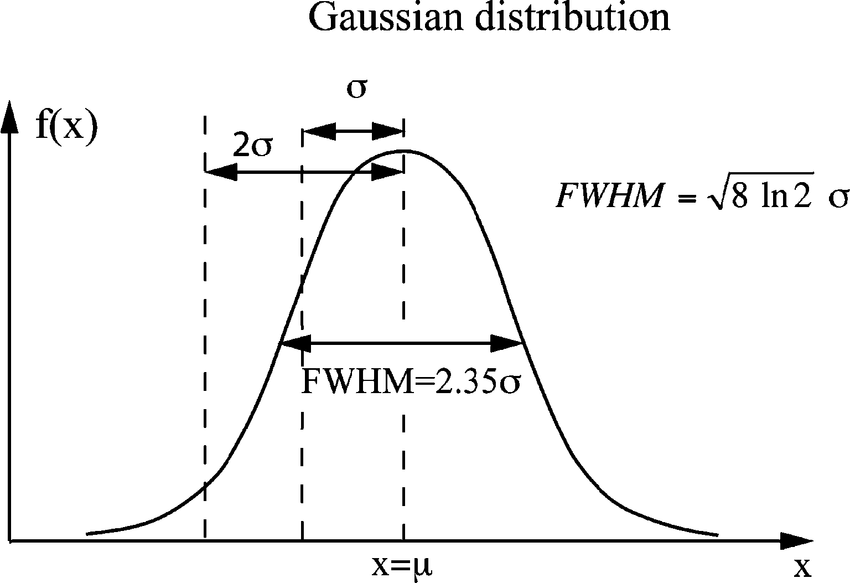
\includegraphics[width=0.6\linewidth]{img//chapter4/fwhm.png}
    \caption[Gaussian PSF and FWHM]{Gaussian or normal PSF and the link with the FWHM.\\\small{Credits: \cite{tavernier_experimental_2010}.}}
    \label{fig:fwhm}
\end{figure}